\chapter{تغيّرات طور مادة نقية}\label{ch:b1:phase-changes}

الماء هو المادة الوحيدة التي رآها الجميع في الحالات الثلاث،
وهو المائع العامل في معظم محطات التوليد في العالم، \omterm{def:b1:heat-engines:vapourcycle}{والمائع
المبرِّد} في أوائل آلات الثلج، ومحرك الطقس.
والجليد ينصهر عند \omterm{def:b1:kinetic-theory:temperature}{درجة حرارة} لا تتزحزح والحرارة تنهال
عليه؛ والغلاية تغلي عند \qty{100}{\degreeCelsius} على شاطئ البحر وعند
\qty{70}{\degreeCelsius} على إفرست؛ وقارورة محكمة فيها ماء شديد البرودة
تتجمد بضربة خفيفة. ويرسم هذا الفصل خريطة أطوار
\omterm{def:b1:phase-changes:phase}{مادة نقية} --- أي مخططَي $(T, P)$ و $(v, P)$ --- ويعطي
الأدوات الثلاث التي ترافقها: \omterm{thm:b1:phase-changes:lever}{قاعدة الرافعة} (كم من كل \omterm{def:b1:phase-changes:phase}{طور})،
\omterm{def:b1:phase-changes:phase}{والحرارة الكامنة} (كم يكلّف التغيّر، طاقةً وإنتروبيا)، \omterm{thm:b1:phase-changes:clapeyron}{وعلاقة
كلاوزيوس-كلابيرون} (كيف تميل خطوط الحدود). وينتهي حيث
تخفق الخريطة: عند \omterm{def:b1:phase-changes:metastable}{الحالات شبه المستقرة}، ومنها يأتي الطقس
ومفاجآت قِدر الضغط.

\section{الأطوار ومخطط $(T, P)$}

\begin{definition}[المادة النقية والطور وتغيّر الطور]\label{def:b1:phase-changes:phase}
\index{طور}\index{تغيّر طور}\index{مادة نقية}\index{حرارة كامنة}
\emph{المادة النقية} جسم من نوع كيميائي واحد. و\emph{الطور}
جزء منها متجانس في خواصه الفيزيائية: صلب أو سائل أو غاز
(ويُسمّى \emph{بخارًا} حين يتعايش مع سائله). و\emph{تغيّر الطور}
(انصهار/تجمّد، تبخّر/تكاثف، تسامٍ/ترسّب) هو الانتقال من طور
إلى آخر؛ ويقع عند ضغط ثابت عند \omterm{def:b1:kinetic-theory:temperature}{درجة حرارة} ثابتة، مع تبادل
حرارة بلا تغيّر في \omterm{def:b1:kinetic-theory:temperature}{درجة الحرارة}: هي \emph{الحرارة الكامنة}.
\end{definition}

\begin{proposition}[مخطط التوازن]\label{prop:b1:phase-changes:PTdiagram}
\index{مخطط الأطوار}\index{النقطة الثلاثية}\index{النقطة الحرجة}\index{ضغط البخار المشبع}
في المستوي $(T, P)$ يشغل كل \omterm{def:b1:phase-changes:phase}{طور} منطقة؛ ولا يتعايش طوران
إلا على منحنٍ (تسامٍ، انصهار، تبخّر)، ولا تتعايش الثلاثة إلا
عند نقطة واحدة، هي \emph{\omterm{prop:b1:phase-changes:PTdiagram}{النقطة الثلاثية}}. ومنحني التبخّر
$P = P_s(T)$ --- وهو \emph{\omterm{prop:b1:phase-changes:PTdiagram}{ضغط البخار المشبع}} --- ينتهي عند
\emph{\omterm{prop:b1:phase-changes:PTdiagram}{النقطة الحرجة}} $(T_c, P_c)$، ولا يبقى السائل والغاز
متمايزين وراءها. وفي الماء: \omterm{prop:b1:phase-changes:PTdiagram}{النقطة الثلاثية} \qty{273.16}{K} و\qty{611}{Pa}؛
\omterm{prop:b1:phase-changes:PTdiagram}{والنقطة الحرجة} \qty{647}{K} و\qty{221}{bar}. ومنحني انصهار الماء
يميل إلى اليسار (فالجليد أقل كثافة من الماء)؛ أما في كل مادة
أخرى تقريبًا فيميل إلى اليمين.
\end{proposition}
\admitted

\begin{omfigure}
\begin{tikzpicture}[font=\small, x=1cm, y=1cm, >=Stealth]
  \draw[->] (0,0) -- (8.4,0) node[below] {$T$};
  \draw[->] (0,0) -- (0,5.2) node[left] {$P$};
  \coordinate (Tp) at (2.4,1.2);
  \coordinate (C) at (6.8,4.4);
  \draw[omDef, very thick] (0.3,0.08) .. controls (1.4,0.3) .. (Tp);
  \draw[omThm, very thick] (Tp) .. controls (2.2,2.8) .. (1.9,5.0);
  \draw[omProp, very thick] (Tp) .. controls (4.6,1.6) and (6.0,3.0) .. (C);
  \fill (Tp) circle (2pt) node[below right, font=\footnotesize] {النقطة الثلاثية $\mathrm T$};
  \fill (C) circle (2pt) node[above left, font=\footnotesize] {النقطة الحرجة $\mathrm C$};
  \node at (0.9,3.4) {صلب};
  \node at (3.6,4.0) {سائل};
  \node at (6.6,0.9) {غاز};
  \node[omDef, font=\footnotesize, anchor=north] at (1.3,0.9) {تسامٍ};
  \node[omThm, font=\footnotesize, rotate=80] at (1.8,3.3) {انصهار};
  \node[omProp, font=\footnotesize, rotate=35] at (5.35,1.9) {تبخّر};
  \draw[dashed] (0,2.4) node[left, font=\footnotesize] {\qty{1}{atm}} -- (8.0,2.4);
  \fill (2.25,2.4) circle (1.6pt) node[above left, font=\footnotesize, xshift=2pt] {\qty{0}{\degreeCelsius}};
  \fill (5.12,2.42) circle (1.6pt) node[above left, font=\footnotesize] {\qty{100}{\degreeCelsius}};
  \draw[dotted] (C) -- (6.8,0) node[below, font=\footnotesize] {$T_c$};
  \node[font=\footnotesize, align=center] at (7.6,3.3) {مائع\\ فوق حرج};
\end{tikzpicture}

{\small مخطط أطوار الماء (لا بمقياس). ويتبع التسخين عند
الضغط الجوي متساوي الضغط المتقطع: فينصهر الجليد حيث
يقطع منحني الانصهار، ويغلي الماء حيث يقطع منحني
التبخّر. ومنحني انصهار الماء يميل إلى اليسار: فالضغط يخفض درجة
انصهاره.}
\end{omfigure}

\begin{remark}[الغليان والتبخّر السطحي وقِدر الضغط]\label{rem:b1:phase-changes:boiling}
\emph{يتبخر} السائل عند أيّ \omterm{def:b1:kinetic-theory:temperature}{درجة حرارة} من سطحه، ما دام
الضغط الجزئي لبخاره فوقه دون $P_s(T)$؛ و\emph{يغلي}
حين يبلغ $P_s(T)$ الضغطَ المحيط، فتستطيع فقاعات
البخار أن تنمو في داخله. والماء يغلي عند \qty{100}{\degreeCelsius}
لأن $P_s(\qty{100}{\degreeCelsius}) = \qty{1.013}{bar}$؛ وعند
\qty{0.33}{bar} على إفرست يغلي قرب \qty{70}{\degreeCelsius}، وفي
قِدر ضغط عند \qty{1.8}{bar} قرب \qty{117}{\degreeCelsius}. \omterm{def:b1:kinetic-theory:temperature}{ودرجة
حرارة} سائل يغلي يثبّتها الضغط --- وهي واقعة
استُعملت لتعريف سلّم سيلزيوس قرنين من الزمان.
\end{remark}

\section{مخطط $(v, P)$ وقاعدة الرافعة}

\begin{proposition}[متساويات حرارة أندروز]\label{prop:b1:phase-changes:andrews}
\index{متساويات حرارة أندروز}\index{منحني التشبع}
في مستوي كلابيرون $(v, P)$ للحجم النوعي، يكون لمتساوي حرارة
$T < T_c$ ثلاثة أجزاء: فرع شديد الميل (وهو السائل، الذي يكاد
لا ينضغط)، و\emph{مسطّح} أفقي عند $P = P_s(T)$ يتعايش فيه السائل
والبخار، وفرع شبيه بقطع زائد (وهو البخار). وطرفا المسطّح
هما الحجمان النوعيان $v_l(T)$ و $v_v(T)$ للسائل والبخار
المشبعين؛ ومحلّهما هو \emph{\omterm{prop:b1:phase-changes:andrews}{منحني التشبع}} (أي
القبة)، وقمته \omterm{prop:b1:phase-changes:PTdiagram}{النقطة الحرجة}، حيث يكون لمتساوي الحرارة $T_c$
انعطاف أفقي. ولا وجود لمسطّح فوق $T_c$.
\end{proposition}
\admitted

\begin{theorem}[قاعدة الرافعة]\label{thm:b1:phase-changes:lever}
\index{قاعدة الرافعة}\index{نسبة البخار}
كتلة $m$ حجمها النوعي $v$ على المسطّح عند $T$ تنقسم إلى
نسبة كتلية بخارية $x = m_v/m$ (وهي \emph{\omterm{thm:b1:phase-changes:lever}{نسبة البخار}}) ونسبة
سائلة $1 - x$ مع
\[
v = (1 - x)v_l + x\,v_v , \qquad\text{أي}\qquad
x = \frac{v - v_l}{v_v - v_l} = \frac{LM}{LV} ,
\]
وهي نسبة القطعتين اللتين تقطعهما نقطة الحالة $M$ على المسطّح.
وتصحّ القاعدة نفسها من أجل كل مقدار امتدادي لواحدة الكتلة ($u$
و $h$ و $s$): $h = (1 - x)h_l + xh_v$.
\end{theorem}

\begin{proof}
الحجوم تتجمع: $V = m_lv_l + m_vv_v$؛ فاقسم على $m$. والطاقة \omterm{def:b1:first-law:enthalpy}{والإنثالبي}
والإنتروبيا امتدادية كذلك.
\end{proof}

\begin{omfigure}
\begin{tikzpicture}[font=\small, x=1cm, y=1cm, >=Stealth]
  \draw[->] (0,0) -- (9.4,0) node[below] {$v$};
  \draw[->] (0,0) -- (0,5.4) node[left] {$P$};
  % dome
  \draw[omDef, thick] plot[smooth, tension=0.8] coordinates {(0.7,0.2) (0.8,2.0) (1.3,3.6) (2.6,4.5) (4.0,3.5) (5.2,2.0) (7.0,1.1) (9.0,0.5)};
  \fill (2.6,4.5) circle (2pt) node[above, font=\footnotesize] {$\mathrm C$};
  % isotherm T1 < Tc
  \draw[omProp, thick] (0.62,5.0) .. controls (0.7,3.2) .. (0.8,2.0) -- (5.2,2.0)
        .. controls (6.4,1.6) and (7.6,1.1) .. (9.2,0.85);
  \node[omProp, font=\footnotesize, anchor=west] at (9.0,1.2) {$T_1$};
  % critical isotherm
  \draw[omThm, thick] (1.1,5.3) .. controls (1.8,4.6) and (2.2,4.5) .. (2.6,4.5)
        .. controls (3.6,4.5) and (5.0,3.4) .. (9.2,2.4);
  \node[omThm, font=\footnotesize, anchor=west] at (9.0,2.7) {$T_c$};
  % supercritical isotherm
  \draw[omExo, thick] (1.7,5.4) .. controls (2.6,4.9) and (4.0,4.4) .. (9.2,3.6);
  \node[omExo, font=\footnotesize, anchor=west] at (9.0,3.9) {$T_2 > T_c$};
  % lever
  \fill (0.8,2.0) circle (1.6pt) node[above left, font=\footnotesize] {$L$};
  \fill (5.2,2.0) circle (1.6pt) node[above right, font=\footnotesize] {$V$};
  \fill (2.5,2.0) circle (1.6pt) node[above, font=\footnotesize] {$M$};
  \draw[<->, omDef] (0.8,1.55) -- (2.5,1.55) node[midway, below, font=\footnotesize] {$x\,(v_v - v_l)$};
  \draw[<->, omDef] (2.5,1.55) -- (5.2,1.55) node[midway, below, font=\footnotesize] {$(1 - x)(v_v - v_l)$};
  \draw[dashed] (0.8,2.0) -- (0.8,0) node[below, font=\footnotesize] {$v_l$};
  \draw[dashed] (5.2,2.0) -- (5.2,0) node[below, font=\footnotesize] {$v_v$};
  \draw[dashed] (2.5,2.0) -- (2.5,0) node[below, font=\footnotesize] {$v$};
  \node[font=\footnotesize, rotate=90] at (0.3,3.4) {سائل};
  \node[font=\footnotesize] at (3.7,0.6) {سائل وبخار};
  \node[font=\footnotesize] at (7.6,0.25) {بخار};
  \draw[dashed] (0,2.0) node[left, font=\footnotesize] {$P_s(T_1)$} -- (0.8,2.0);
\end{tikzpicture}

{\small \omterm{prop:b1:phase-changes:andrews}{متساويات حرارة أندروز} في مخطط كلابيرون. فتحت القبة
يكون متساوي الحرارة $T_1$ مسطّحًا عند $P_s(T_1)$؛ وتكون حالة $M$ عليه
مزيجًا نسبته البخارية $x$ هي النسبة $LM/LV$. ويلامس متساوي الحرارة
الحرج القبةَ عند قمتها بانعطاف أفقي؛
وفوق $T_c$ لا مسطّح ولا تمايز بين السائل
والغاز.}
\end{omfigure}

\begin{example}[غلاية ومِرجل]\label{ex:b1:phase-changes:lever}
الماء عند \qty{100}{\degreeCelsius} و\qty{1}{atm}: $v_l = \qty{1.04e-3}{m^3/kg}$
و $v_v = \qty{1.67}{m^3/kg}$ --- أي بنسبة $1600$. ووعاء مغلق سعته \qty{1.0}{L}
فيه \qty{0.50}{kg} من الماء عند تلك الدرجة له $v =
\qty{2.0e-3}{m^3/kg}$ و $x = (2.0 - 1.04) \times 10^{-3}/1.67 = 5.8 \times 10^{-4}$:
أي \qty{0.29}{g} من البخار تشغل نصف الوعاء. ومضاعفة كتلة البخار
في وعاء محكم لا تكاد تزحزح نقطة الحالة؛ فالضغط
تعيّنه \omterm{def:b1:kinetic-theory:temperature}{درجة الحرارة} وحدها.
\end{example}

\section{طاقيات تغيّر الطور}

\begin{proposition}[الحرارة الكامنة وإنثالبي التحول وإنتروبيته]\label{prop:b1:phase-changes:latent}
\index{إنثالبي التحول}\index{إنتروبيا التحول}
عند \omterm{def:b1:kinetic-theory:temperature}{درجة الحرارة} $T$ وضغط التعايش $P_s(T)$، يكون
تحول واحدة الكتلة من \omterm{def:b1:phase-changes:phase}{الطور} 1 إلى \omterm{def:b1:phase-changes:phase}{الطور} 2 عكوسًا،
ومتساوي الحرارة ومتساوي الضغط، ويكون
\[
L_{12}(T) = h_2 - h_1 , \qquad s_2 - s_1 = \frac{L_{12}}{T} , \qquad
u_2 - u_1 = L_{12} - P_s(v_2 - v_1) .
\]
حيث $L_{12} > 0$ في الانتقال نحو \omterm{def:b1:phase-changes:phase}{الطور} الأقل انتظامًا (الانصهار
والتبخّر والتسامي)، ويكون $L_{21} = -L_{12}$. وفي الماء عند \qty{1}{atm}:
$L_f = \qty{334}{kJ/kg}$ عند \qty{0}{\degreeCelsius}، و $L_v = \qty{2257}{kJ/kg}$ عند
\qty{100}{\degreeCelsius}.
\end{proposition}

\begin{proof}
تكون الحرارة المتلقاة عند ثبات الضغط هي $\Delta H$
(\cref{prop:b1:first-law:qvqp})؛ وهي، بكونه عكوسًا ومتساوي الحرارة،
$T\Delta S$ (\cref{prop:b1:second-law-entropy:identity})؛ ولدينا $U = H - PV$.
\end{proof}

\begin{example}[أين تذهب حرارة التبخّر]\label{ex:b1:phase-changes:whereheat}
في الماء عند \qty{100}{\degreeCelsius}: $P_s(v_v - v_l) = 1.013 \times 10^5 \times
1.67 = \qty{169}{kJ/kg}$، ومنه $u_v - u_l = 2257 - 169 = \qty{2088}{kJ/kg}$:
فيذهب $93\%$ من \omterm{def:b1:phase-changes:phase}{الحرارة الكامنة} إلى تمزيق الجزيئات بعضها عن بعض، و $7\%$
إلى دفع الجوّ إلى الوراء. وإنتروبيا التبخّر،
$2257/373 = \qty{6.05}{kJ/(kg.K)}$، تقزّم إنتروبيا الانصهار، $334/273 =
\qty{1.22}{kJ/(kg.K)}$: فالانصهار يرخي الجزيئات، والغليان يحرّرها.
\end{example}

\begin{method}[المسعرية مع تغيّرات الطور]\label{meth:b1:phase-changes:calorimetry}
في وعاء معزول عند ضغط ثابت يكون $\sum\Delta H_i = 0$. فخمّن
الحالة النهائية (أيّ الأطوار حاضر، وعند أيّ \omterm{def:b1:kinetic-theory:temperature}{درجة حرارة})؛
واكتب $\Delta H$ لكل جسم بوصفها حرارات محسوسة $mc\,\Delta T$ زائد حرارات
كامنة $\pm mL$ للتغيّرات التي يمرّ بها؛ ثم حُلّ؛ و\emph{تحقّق من
التخمين}: فجسم ينتهي فوق درجة غليانه أو دون درجة انصهاره،
أو كتلة سالبة \omterm{def:b1:phase-changes:phase}{لطور}، يعني أن التخمين كان خطأ --- وتكون
الحالة النهائية عندئذ مزيجًا عند \omterm{def:b1:kinetic-theory:temperature}{درجة حرارة} التحول، ويصير
المجهول هو الكتلة المتحولة (\cref{ex:b1:first-law:ice}).
\end{method}

\begin{example}[حروق البخار]\label{ex:b1:phase-changes:steam}
\qty{10}{g} من البخار عند \qty{100}{\degreeCelsius} تتكاثف على الجلد فتعطي
$0.010 \times 2257 = \qty{22.6}{kJ}$ قبل أن تبرد درجة واحدة ---
أي بقدر ما تعطيه \qty{10}{g} من الماء المغلي وهي تبرد بمقدار
\qty{540}{K}. ولهذا يسلخ البخار أشدّ بكثير من الماء عند الدرجة
نفسها، ولهذا يحتاج مشعّ بخاري إلى تدفق كتلي ضئيل.
\end{example}

\begin{omfigure}
\begin{tikzpicture}[font=\small, x=1cm, y=1cm, >=Stealth]
  \draw[->] (0,0) -- (9.0,0) node[below] {$s$};
  \draw[->] (0,0) -- (0,5.2) node[left] {$T$};
  \draw[omDef, thick] (0.9,0.3) .. controls (1.3,2.6) and (2.6,4.4) .. (4.0,4.6)
        .. controls (5.4,4.4) and (7.0,2.4) .. (8.4,0.3);
  \fill (4.0,4.6) circle (2pt) node[above, font=\footnotesize] {$\mathrm C$};
  % isobar at T1
  \draw[omProp, thick] (0.6,0.35) .. controls (1.1,1.2) .. (1.65,2.6) -- (6.65,2.6)
        .. controls (7.4,3.0) and (8.0,3.6) .. (8.6,4.5);
  \node[omProp, font=\footnotesize, anchor=west] at (8.6,4.6) {متساوي الضغط $P_1$};
  \draw[dashed] (1.65,2.6) -- (1.65,0) node[below, font=\footnotesize] {$s_l$};
  \draw[dashed] (6.65,2.6) -- (6.65,0) node[below, font=\footnotesize] {$s_v$};
  \draw[dashed] (0,2.6) node[left, font=\footnotesize] {$T_1$} -- (1.65,2.6);
  \draw[<->, omThm] (1.65,2.9) -- (6.65,2.9) node[midway, above, font=\footnotesize] {$s_v - s_l = L_v/T_1$};
  \fill[omThm!15] (1.65,0) rectangle (6.65,2.6);
  \node[font=\footnotesize, omThm] at (4.15,1.2) {المساحة $= L_v$};
  \node[font=\footnotesize] at (1.0,3.9) {سائل};
  \node[font=\footnotesize] at (8.3,1.9) {بخار};
  \node[font=\footnotesize] at (4.15,2.0) {سائل وبخار};
\end{tikzpicture}

{\small القبة نفسها في \omterm{def:b1:second-law-entropy:TS}{مخطط الإنتروبيا}. يقطعها متساوي ضغط
في قطعة أفقية طولها $L_v/T$؛ والمساحة تحت القطعة هي
\omterm{def:b1:phase-changes:phase}{الحرارة الكامنة}. وتُرسم أدوار محطات التوليد في هذا المستوي، وتُقرأ
\omterm{thm:b1:phase-changes:lever}{نسبة البخار} عند مخرج العنفة على القطعة \omterm{thm:b1:phase-changes:lever}{بقاعدة
الرافعة}.}
\end{omfigure}

\section{علاقة كلاوزيوس-كلابيرون}

\begin{theorem}[كلاوزيوس-كلابيرون]\label{thm:b1:phase-changes:clapeyron}
\index{علاقة كلاوزيوس-كلابيرون}
على امتداد منحني تعايش الطورين 1 و 2، يكون
\[
\frac{\dd P_s}{\dd T} = \frac{L_{12}(T)}{T\,(v_2 - v_1)} .
\]
\end{theorem}

\begin{proof}
أدر واحدة الكتلة في \omterm{def:b1:heat-engines:carnotcycle}{دور كارنو} تفاضلي داخل القبة:
تحول تامّ $1 \to 2$ على امتداد المسطّح عند $T + \dd T$ وعند الضغط
$P_s + \dd P_s$ (فالحرارة المتلقاة $L_{12}$ إلى المرتبة الأولى)؛ ثم خطوة
كظومة تفاضلية نزولًا إلى $T$؛ ثم التحول العكسي على امتداد المسطّح عند
$T$ و $P_s$؛ ثم خطوة كظومة عائدة. والدور عكوس، ثنائي المنبع
بين $T + \dd T$ و $T$، فيكون مردوده $\dd T/T$
(\cref{thm:b1:heat-engines:carnot})؛ وشغله، وهو مساحة المستطيل
الرفيع، هو $\dd P_s\,(v_2 - v_1)$. ومنه $\dd P_s\,(v_2 - v_1)/L_{12} =
\dd T/T$.
\end{proof}

\begin{omfigure}
\begin{tikzpicture}[font=\small, x=1cm, y=1cm, >=Stealth]
  \draw[->] (0,0) -- (8.6,0) node[below] {$v$};
  \draw[->] (0,0) -- (0,4.6) node[left] {$P$};
  \draw[omDef, thick] (0.6,0.2) .. controls (0.75,2.0) and (1.6,3.7) .. (2.6,4.0)
        .. controls (3.6,3.7) and (5.8,1.6) .. (8.2,0.4);
  \fill[omProp!25] (0.92,2.0) -- (4.88,2.0) -- (4.95,2.3) -- (0.9,2.3) -- cycle;
  \draw[omProp, thick] (0.92,2.0) -- (4.88,2.0) node[pos=0.5, below, font=\footnotesize] {$T$, $P_s$};
  \draw[omThm, thick] (0.9,2.3) -- (4.95,2.3) node[pos=0.5, above, font=\footnotesize] {$T + \dd T$, $P_s + \dd P_s$};
  \draw[<->] (6.2,2.0) -- (6.2,2.3) node[midway, right, font=\footnotesize] {$\dd P_s$};
  \draw[dotted] (4.88,2.0) -- (6.3,2.0); \draw[dotted] (4.95,2.3) -- (6.3,2.3);
  \draw[<->] (0.92,1.4) -- (4.88,1.4) node[midway, below, font=\footnotesize] {$v_2 - v_1$};
  \draw[dotted] (0.92,2.0) -- (0.92,1.3); \draw[dotted] (4.88,2.0) -- (4.88,1.3);
  \node[font=\footnotesize, omProp, anchor=west] at (4.0,3.5) {$-W = \dd P_s\,(v_2 - v_1)$, \; $Q_h = L_{12}$};
\end{tikzpicture}

{\small \omterm{def:b1:heat-engines:carnotcycle}{دور كارنو} التفاضلي الذي يبرهن على \omterm{thm:b1:phase-changes:clapeyron}{علاقة
كلاوزيوس-كلابيرون}: مسطّحان يفصل بينهما $\dd T$، تصل بينهما
خطوتان كظومتان أقصر من أن تُرسما؛ وتساوي \omterm{thm:b1:heat-engines:carnot}{مبرهنة كارنو} بين نسبة
مساحته إلى الحرارة المتلقاة والمقدار $\dd T/T$.}
\end{omfigure}

\begin{corollary}[ضغط البخار المشبع لسائل]\label{cor:b1:phase-changes:vapourpressure}
إذا كان البخار غازًا مثاليًّا و $v_v \gg v_l$، بحيث يكون $v_v - v_l \approx
RT/(MP_s)$، وإذا تغيّرت $L_v$ قليلًا، فإن
\[
\frac{\dd P_s}{P_s} = \frac{ML_v}{R}\,\frac{\dd T}{T^2} , \qquad
\ln\frac{P_s(T)}{P_s(T_0)} = \frac{ML_v}{R}\Bigl(\frac{1}{T_0} - \frac{1}{T}\Bigr) :
\]
أي أن ضغط البخار يرتفع ارتفاعًا أسّيًّا تقريبًا مع \omterm{def:b1:kinetic-theory:temperature}{درجة الحرارة}. وفي
الماء قرب \qty{100}{\degreeCelsius}: $ML_v/R = 0.018 \times 2.257 \times 10^6/
8.314 = \qty{4890}{K}$ و $\dd P_s/\dd T = 2.257 \times 10^6/(373 \times 1.67) =
\qty{3.6}{kPa/K}$: فكل \omterm{def:b1:kinetic-theory:temperature}{كلفن} إضافي في درجة الغليان يكلّف
\qty{36}{mbar} من الضغط الإضافي.
\end{corollary}

\begin{proof}
عوّض $v_v - v_l \approx RT/(MP_s)$ في المبرهنة وافصل
المتغيرات؛ ثم كامل مع $L_v$ ثابتة.
\end{proof}

\begin{omfigure}
\begin{tikzpicture}
\begin{axis}[omaxis, axis x line=bottom, axis y line=left, width=10.5cm, height=6.2cm,
    xlabel={$T$ (\unit{\degreeCelsius})}, ylabel={$P_s$ (\unit{kPa})},
    xlabel style={at={(axis description cs:0.5,-0.14)}, anchor=north},
    xmin=0, xmax=130, ymin=0, ymax=230, xtick={0,20,...,120}, ytick={50,100,150,200}, samples=120, clip=false]
  \addplot[omDef, thick, domain=0:125] {0.133322*10^(8.07131-1730.63/(233.426+x))};
  \addplot[black, dashed] coordinates {(0,101.3) (100,101.3) (100,0)};
  \addplot[black, dashed] coordinates {(0,33) (71,33) (71,0)};
  \addplot[black, dashed] coordinates {(0,180) (117,180) (117,0)};
  \node[font=\footnotesize, anchor=south west] at (axis cs:2,103) {سطح البحر: \qty{100}{\degreeCelsius}};
  \node[font=\footnotesize, anchor=south west] at (axis cs:2,35) {إفرست (\qty{0.33}{bar}): \qty{71}{\degreeCelsius}};
  \node[font=\footnotesize, anchor=south west] at (axis cs:2,182) {قِدر الضغط (\qty{1.8}{bar}): \qty{117}{\degreeCelsius}};
\end{axis}
\end{tikzpicture}

{\small \omterm{prop:b1:phase-changes:PTdiagram}{ضغط البخار المشبع} للماء. والمنحني قريب من
أسّي في $-1/T$؛ ودرجة الغليان هي حيث يقطع
الضغطَ المحيط.}
\end{omfigure}

\begin{example}[الجليد تحت المزلج]\label{ex:b1:phase-changes:skate}
في الجليد والماء: $L_f = \qty{334}{kJ/kg}$ و $v_l - v_s = (1.000 - 1.091)
\times 10^{-3} = \qty{-9.1e-5}{m^3/kg}$: ومنه $\dd P/\dd T = 3.34 \times 10^5/(273 \times
(-9.1 \times 10^{-5})) = \qty{-1.3e7}{Pa/K} = \qty{-130}{bar/K}$. ومتزلج كتلته \qty{70}{kg}
على نصل واحد أبعاده \qty{30}{cm} في \qty{3}{mm} ($\qty{9}{cm^2}$) يؤثر
بنحو \qty{8}{bar}، فيخفض درجة الانصهار بمقدار \qty{0.06}{K} --- فليس الانصهار بالضغط هو سبب انزلاق المزالج (إذ إن طبقة
سطحية رفيعة من الجليد تشبه السائل من تلقائها، والاحتكاك يسخّن)؛
لكن الميل السالب حقيقي، وهو سبب أن سلكًا محمَّلًا
بأثقال يشقّ كتلة جليد تتجمد من جديد خلفه.
\end{example}

\section{الحالات شبه المستقرة}

\begin{definition}[التبريد الفائق والتسخين الفائق]\label{def:b1:phase-changes:metastable}
\index{تبريد فائق}\index{تسخين فائق}\index{حالة شبه مستقرة}\index{تنوّي}
يمكن \omterm{def:b1:phase-changes:phase}{لطور} أن يدوم وراء حدّ توازنه: فالماء السائل
يُبرَّد دون \qty{0}{\degreeCelsius} بلا تجمّد (وهو \emph{التبريد الفائق})،
ويُسخَّن فوق درجة غليانه بلا غليان (وهو \emph{التسخين الفائق})،
ويُضغط البخار وراء $P_s$ بلا تكاثف (وهو التشبع الفائق).
وتقتضي مثل هذه \emph{الحالات شبه المستقرة} غياب مواقع
\emph{التنوّي} --- الغبار، والخدوش، والغاز المنحلّ، وبلورات الجليد --- التي
يستطيع \omterm{def:b1:phase-changes:phase}{الطور} الجديد أن يبدأ عليها؛ وأيّ اضطراب يقلبها فجأةً ولاعكوسيًّا
إلى التوازن.
\end{definition}

\begin{example}[القارورة المبرَّدة تبريدًا فائقًا]\label{ex:b1:phase-changes:supercooled}
ماء ساكن عند \qty{-8}{\degreeCelsius} في قارورة نظيفة، تُطرَق: فتنطلق
بلورات الجليد خلاله وتقفز \omterm{def:b1:kinetic-theory:temperature}{درجة الحرارة} إلى
\qty{0}{\degreeCelsius}. والسيرورة كظومة وسريعة، فتجمّد الحرارة
المحسوسة $c\,\Delta T$ النسبةَ $x = c\,\Delta T/L_f = 4.18 \times 8/334 =
0.10$ من الماء؛ والإنتروبيا المُنشأة، $c\ln(273/265) - xL_f/273 =
124 - 122 = \qty{+2}{J/(kg.K)}$، موجبة كما يجب. والغيوم
مملوءة بقطيرات مبرَّدة تبريدًا فائقًا حتى \qty{-40}{\degreeCelsius}؛ ويستغل ذلك
تجمّدُ الطائرات وتلقيحُ الغيوم كلاهما.
\end{example}

\begin{remark}[حصى الغليان وحجرات الفقاعات]\label{rem:b1:phase-changes:nucleation}
فقاعة نصف قطرها $r$ في سائل عند الضغط $P$ تحوي بخارًا عند
$P + 2\sigma/r$ (حيث $\sigma$ التوتر السطحي، في مجلد السنة الثانية)؛ ولا تستطيع
أن تنمو إلا إذا كان $P_s(T) > P + 2\sigma/r$، فلا يكون في سائل نظيف عند درجة غليانه
فقاعة صغيرة كفايةً لتبدأ، فيُسخَّن تسخينًا فائقًا ببضعة كلفنات
قبل أن يثور --- وهو ``النطّ'' الذي تمنعه حصى الغليان بأن
تقدّم تجاويف مملوءة بغاز محتبس. وحجرة الفقاعات في فيزياء
الجسيمات كانت تعمل على عدم الاستقرار نفسه معكوسًا: فالسائل المسخَّن تسخينًا فائقًا
يغلي أولًا على امتداد أثر جسيم مؤيِّن.
\end{remark}

\begin{example}[الرطوبة والندى]\label{ex:b1:phase-changes:dew}
\index{رطوبة نسبية}\index{نقطة الندى}
يحمل الهواء بخار ماء عند ضغط جزئي $P_v \leq P_s(T)$؛ و\emph{\omterm{ex:b1:phase-changes:dew}{الرطوبة
النسبية}} هي $P_v/P_s(T)$، و\emph{\omterm{ex:b1:phase-changes:dew}{نقطة الندى}} هي
\omterm{def:b1:kinetic-theory:temperature}{درجة الحرارة} التي يهبط عندها $P_s$ إلى $P_v$. فهواء عند \qty{25}{\degreeCelsius}
($P_s = \qty{3.17}{kPa}$) برطوبة $60\%$ له $P_v = \qty{1.9}{kPa}$
و $\rho_v = P_vM/(RT) = \qty{14}{g/m^3}$، ويتندّى على أيّ سطح دون
\qty{17}{\degreeCelsius} تقريبًا --- على العشب عند الفجر، وعلى القارورة الباردة، وعلى
مرآة الحمّام. وإذا ارتفع الهواء نفسه برد كظومًا بمعدل
\qty{9.8}{K/km} (\cref{pb:b1:phase-changes:1}) وبلغ نقطة ندائه على ارتفاع
كيلومتر أو نحوه: وهناك تكون القيعان المسطّحة للسحب الركامية.
\end{example}

\section{تمارين}

\begin{exercise}[$\star$]\label{exo:b1:phase-changes:1}
باستعمال مخطط الدرس، أعطِ \omterm{def:b1:phase-changes:phase}{طور} الماء (أ) عند
\qty{20}{\degreeCelsius} تحت \qty{0.5}{kPa}؛ (ب) عند \qty{-5}{\degreeCelsius}
تحت \qty{1}{bar}؛ (ج) عند \qty{400}{\degreeCelsius} تحت \qty{200}{bar}؛
(د) عند \qty{0.01}{\degreeCelsius} تحت \qty{611}{Pa}. ولماذا تجفّ بركة
عند \qty{20}{\degreeCelsius} مع أن الماء ``يغلي عند 100''؟
\end{exercise}

\begin{exercise}[$\star$]\label{exo:b1:phase-changes:2}
\qty{100}{g} من البخار عند \qty{100}{\degreeCelsius} تُفقَّع في
\qty{1.0}{kg} من الماء عند \qty{20}{\degreeCelsius} في وعاء معزول.
أوجد \omterm{def:b1:kinetic-theory:temperature}{درجة الحرارة} النهائية ($L_v = \qty{2257}{kJ/kg}$ و $c = \qty{4.18}{kJ/(kg.K)}$).
وقارن بإضافة \qty{100}{g} من الماء عند \qty{100}{\degreeCelsius}.
\end{exercise}

\begin{exercise}[$\star$]\label{exo:b1:phase-changes:3}
وعاء صلب سعته \qty{2.0}{L} فيه \qty{1.0}{kg} من الماء عند
\qty{150}{\degreeCelsius} في توازن سائل وبخار ($P_s =
\qty{4.76}{bar}$ و $v_l = \qty{1.09e-3}{m^3/kg}$ و $v_v = \qty{0.393}{m^3/kg}$).
أوجد \omterm{thm:b1:phase-changes:lever}{نسبة البخار}، وكتلة البخار، والحجم الذي يشغله السائل.
\end{exercise}

\begin{exercise}[$\star$]\label{exo:b1:phase-changes:4}
إنتروبيا تبخّر الماء عند \qty{100}{\degreeCelsius}، للكيلوغرام
وللمول؛ وإنتروبيا الانصهار \omterm{def:b1:kinetic-theory:scales}{للمول} عند \qty{0}{\degreeCelsius}. ولسوائل
عادية كثيرة إنتروبيا تبخّر مولية قرب
\qty{88}{J/(mol.K)} (وهي قاعدة تروتون): فهل الماء عادي؟
\end{exercise}

\begin{exercise}[$\star\star$]\label{exo:b1:phase-changes:5}
درجة غليان الماء على قمة إفرست، حيث $P =
\qty{0.33}{bar}$، انطلاقًا من \cref{cor:b1:phase-changes:vapourpressure} مع
$ML_v/R = \qty{4890}{K}$؛ ثم عند \qty{2000}{m} (حيث $P = \qty{0.80}{bar}$). وماذا
يصير إلى بيضة تُسلَق \qty{3}{min}؟
\end{exercise}

\begin{exercise}[$\star\star$]\label{exo:b1:phase-changes:6}
\omterm{def:b1:kinetic-theory:temperature}{درجة الحرارة} داخل قِدر ضغط ينفتح صمامه عند \qty{1.8}{bar}
مطلقًا؛ ثم لو ضُبط صمامه على \qty{2.5}{bar}. وللبخار عند
\qty{1.8}{bar} حجم نوعي $v_v = \qty{0.98}{m^3/kg}$: فكم غرامًا من البخار
يحوي قِدر سعته \qty{6}{L} فوق \qty{4}{L} من الماء؟
\end{exercise}

\begin{exercise}[$\star\star$]\label{exo:b1:phase-changes:7}
ميل منحني انصهار الماء عند \qty{0}{\degreeCelsius} ($L_f =
\qty{334}{kJ/kg}$ و $v_s = \qty{1.091e-3}{m^3/kg}$ و $v_l = \qty{1.000e-3}{m^3/kg}$).
وعند أيّ ضغط ينصهر الجليد عند \qty{-1}{\degreeCelsius}؟ وجليد في
أسفل صفيحة جليدية سماكتها \qty{3}{km} ($\rho = \qty{917}{kg/m^3}$): ما درجة
الانصهار هناك، وما نتيجة ذلك في جريان الأنهار الجليدية؟
\end{exercise}

\begin{exercise}[$\star\star$]\label{exo:b1:phase-changes:8}
كيلوغرام واحد من الماء يغلي كله عند \qty{100}{\degreeCelsius} تحت
\qty{1}{atm} ($v_v = \qty{1.673}{m^3/kg}$ و $v_l = \qty{1.04e-3}{m^3/kg}$).
أوجد الشغل المتلقى والحرارة المتلقاة و $\Delta U$ و $\Delta H$ و $\Delta S$
للماء؛ والإنتروبيا المُنشأة إن أتت الحرارة من لهب عند
\qty{1500}{K}.
\end{exercise}

\begin{exercise}[$\star\star$]\label{exo:b1:phase-changes:9}
ضغوط التشبع: \qty{1.23}{kPa} عند \qty{10}{\degreeCelsius}، و\qty{1.70}
عند \qty{15}{\degreeCelsius}، و\qty{2.34} عند \qty{20}{\degreeCelsius}، و\qty{3.17}
عند \qty{25}{\degreeCelsius}، و\qty{4.24}{kPa} عند \qty{30}{\degreeCelsius}. وغرفة
عند \qty{22}{\degreeCelsius} رطوبتها النسبية $70\%$: أوجد ضغط
البخار، \omterm{ex:b1:phase-changes:dew}{ونقطة الندى} (بالاستكمال الخطي)، وكتلة بخار الماء في
\qty{50}{m^3}. ولوح نافذة عند \qty{12}{\degreeCelsius}: فهل يتضبّب؟
ثم تُسخَّن الغرفة إلى \qty{25}{\degreeCelsius} بلا إضافة ماء: فما
الرطوبة الجديدة؟
\end{exercise}

\begin{exercise}[$\star\star\star$]\label{exo:b1:phase-changes:10}
\emph{\omterm{prop:b1:phase-changes:PTdiagram}{النقطة الثلاثية}.} (أ) بيّن انطلاقًا من كون $h$ دالة حالة
أنه عند \omterm{prop:b1:phase-changes:PTdiagram}{النقطة الثلاثية} يكون $L_s = L_f + L_v$ (أي التسامي = الانصهار +
التبخّر). (ب) بيّن \omterm{thm:b1:phase-changes:clapeyron}{بعلاقة كلاوزيوس-كلابيرون} أن منحني التسامي
أشدّ ميلًا من منحني التبخّر عند \omterm{prop:b1:phase-changes:PTdiagram}{النقطة الثلاثية}
(بإهمال $v_s$ و $v_l$ أمام $v_v$). (ج) وفي الماء: $L_f = \qty{334}{kJ/kg}$
و $L_v = \qty{2500}{kJ/kg}$ و $T = \qty{273.16}{K}$ و $P = \qty{611}{Pa}$، والبخار
\omterm{def:b1:kinetic-theory:model}{غاز مثالي}: أوجد الميلين بوحدة \unit{Pa/K}. (د) ولماذا يختفي الثلج
في يوم بارد جافّ من دون أن ينصهر أبدًا؟
\end{exercise}

\begin{exercise}[$\star\star\star$]\label{exo:b1:phase-changes:11}
\emph{الماء المسخَّن تسخينًا فائقًا.} فقاعة نصف قطرها $r$ في ماء عند الضغط
$P_0$ تحوي بخارًا عند $P_0 + 2\sigma/r$ مع $\sigma = \qty{0.059}{N/m}$
(مسلَّم به). (أ) أوجد أصغر نصف قطر لفقاعة تستطيع النمو في ماء عند
\qty{105}{\degreeCelsius} تحت \qty{1.013}{bar}، باستعمال
$\dd P_s/\dd T = \qty{3.6}{kPa/K}$. (ب) والسؤال نفسه عند \qty{101}{\degreeCelsius}.
(ج) كوب ماء سُخّن تسخينًا فائقًا إلى \qty{105}{\degreeCelsius} في فرن
ميكروويف تضطربه ملعقة: أوجد نسبة الماء الذي يتبخر فجأةً،
وحجم البخار المنتَج لكل لتر من الماء --- وعلّق
على الخطر. (د) ولماذا تمنع حصى الغليان ذلك؟
\end{exercise}

\begin{exercise}[$\star\star\star$]\label{exo:b1:phase-changes:12}
\emph{دور \omterm{def:b1:heat-engines:vapourcycle}{مائع مبرِّد}.} \omterm{def:b1:heat-engines:machine}{مضخة حرارية} تدير R-134a على
\cref{def:b1:heat-engines:vapourcycle}: التبخّر عند
\qty{-10}{\degreeCelsius} (\qty{2.0}{bar}؛ $h_l = \qty{187}{kJ/kg}$ و $h_v =
\qty{392}{kJ/kg}$)، والتكاثف عند \qty{40}{\degreeCelsius} (\qty{10.2}{bar}؛
$h_l = \qty{256}{kJ/kg}$ و $h_v = \qty{419}{kJ/kg}$). ويغادر المائع
المكثِّف سائلًا مشبعًا والمبخِّر بخارًا مشبعًا؛
ويقدّمه الضاغط عند $h = \qty{430}{kJ/kg}$. وسلّم بأن $h$ ينحفظ في
الصمام وبأن شغل الضاغط للكيلوغرام هو
$\Delta h$ (وهي موازنات الجريان المستقر، في مجلد السنة الثانية)؛ وفي المبادلين،
عند ثبات الضغط، $q = \Delta h$ (\cref{prop:b1:first-law:qvqp}). (أ) أوجد \omterm{thm:b1:phase-changes:lever}{نسبة البخار}
عند مدخل المبخِّر. (ب) والحرارة المأخوذة للكيلوغرام في المبخِّر،
والحرارة المعطاة في المكثِّف، وشغل الانضغاط؛ وتحقّق من المبدأ الأول.
(ج) و $e_p$ و $e_f$؛ وقارنهما بقيمتَي كارنو بين درجتَي
حرارة التشبع. (د) والتدفق الكتلي من أجل \qty{6}{kW} من التدفئة.
\end{exercise}

\begin{omfigure}
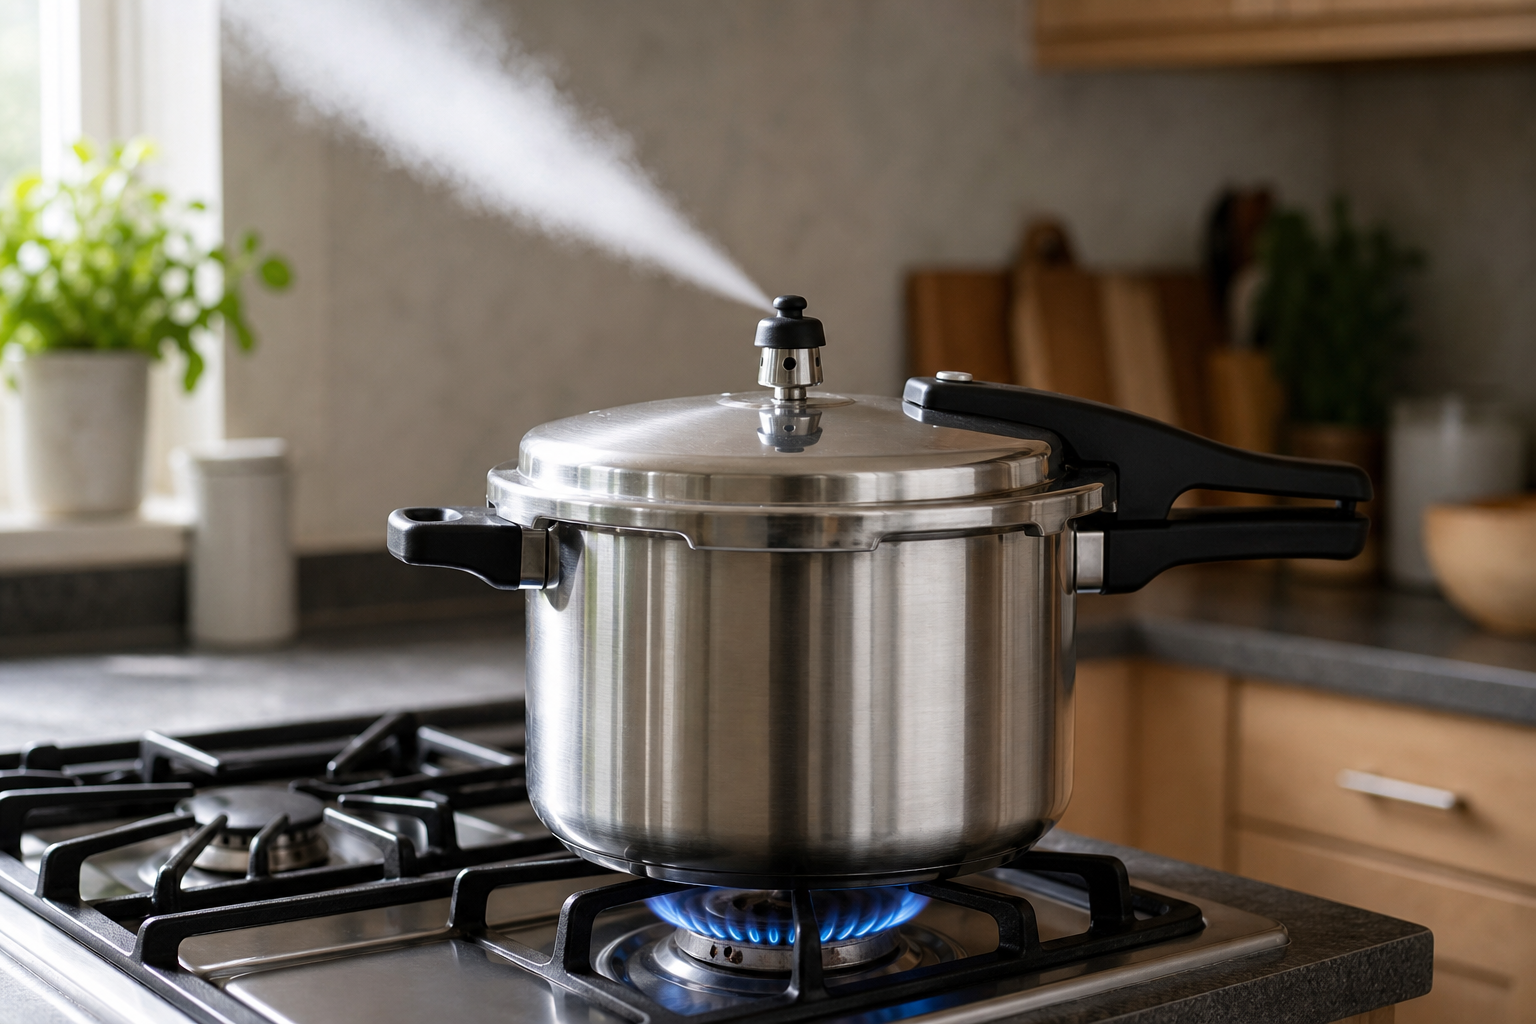
\includegraphics[width=0.58\linewidth]{images/book3/ai/b3-25-pressure-cooker-steam.png}

{\small قِدر ضغط: عند \qty{1.8}{bar} يغلي الماء عند \qty{117}{\degreeCelsius}، والصمام المثقَّل هو الذي يعيّن الضغط.}
\end{omfigure}

\section{مسألة: الماء في أربعة مشاهد}

\begin{problem}[{مسألة نهاية الأسبوع --- قِدر الضغط، والسحابة،
والوعاء المحكم، والقارورة المبرَّدة تبريدًا فائقًا: مادة واحدة وأربعة استعمالات
لمخطط أطوارها}]
\label{pb:b1:phase-changes:1}
معطيات الماء: $L_v = \qty{2257}{kJ/kg}$ عند \qty{100}{\degreeCelsius} ونحو
\qty{2.2}{MJ/kg} عند \qty{117}{\degreeCelsius}، و\qty{2.45}{MJ/kg} قرب
\qty{20}{\degreeCelsius}؛ و $L_f = \qty{334}{kJ/kg}$؛ و $c = \qty{4.18}{kJ/(kg.K)}$
للسائل؛ و $M = \qty{18}{g/mol}$؛ و $ML_v/R = \qty{4890}{K}$ قرب
\qty{100}{\degreeCelsius}. وضغوط التشبع: \qty{0.61}{kPa}
عند \qty{0}{\degreeCelsius}، و\qty{1.23} عند \qty{10}، و\qty{1.70} عند \qty{15}،
و\qty{2.34} عند \qty{20}، و\qty{3.17} عند \qty{25}، و\qty{4.24}{kPa}
عند \qty{30}{\degreeCelsius}، و\qty{101.3}{kPa} عند \qty{100}{\degreeCelsius}.
والحجوم النوعية المشبعة: $v_l = \qty{1.0e-3}{m^3/kg}$ للماء البارد،
و\qty{1.9e-3}{m^3/kg} عند \qty{360}{\degreeCelsius}؛ و $v_v = \qty{0.0217}{m^3/kg}$
عند \qty{300}{\degreeCelsius}، و $0.0108$ عند \qty{340}{\degreeCelsius}، و $0.0088$
عند \qty{350}{\degreeCelsius}؛ \omterm{prop:b1:phase-changes:PTdiagram}{والنقطة الحرجة} \qty{374}{\degreeCelsius}
و\qty{221}{bar} و $v_c = \qty{3.1e-3}{m^3/kg}$. والهواء: $M = \qty{29}{g/mol}$ و $c_p =
\qty{1.0}{kJ/(kg.K)}$ و $\gamma = 1.4$؛ و $g = \qty{9.8}{m/s^2}$؛ و $R =
\qty{8.314}{J/(mol.K)}$.

\medskip
\noindent\textbf{الجزء I --- قِدر الضغط.}
\begin{enumerate}
  \item لماذا لا يمكن تسخين ماء في إناء مفتوح عند سطح البحر فوق
        \qty{100}{\degreeCelsius}، مهما يشتدّ اللهب؟
  \item انطلاقًا من \omterm{thm:b1:phase-changes:clapeyron}{علاقة كلاوزيوس-كلابيرون}، اشتقّ
        $\ln[P_s(T)/P_s(T_0)] = (ML_v/R)(1/T_0 - 1/T)$، مع ذكر
        التقريبات.
  \item \omterm{def:b1:kinetic-theory:temperature}{درجة الحرارة} في قِدر ينفتح صمامه عند \qty{1.8}{bar}
        مطلقًا.
  \item الصمام ثقل يستقر على فتحة مساحتها \qty{20}{mm^2}؛
        والضغط الجوي \qty{1.0}{bar}: فما كتلة الثقل؟
  \item يُرفع \qty{2.0}{L} من الماء من \qty{20}{\degreeCelsius} إلى
        \omterm{def:b1:kinetic-theory:temperature}{درجة حرارة} العمل بصفيحة استطاعتها \qty{2.0}{kW} (أهمل القِدر):
        أوجد الحرارة والزمن.
  \item وبعد بلوغها تُترك الصفيحة عند \qty{2.0}{kW}: فما كتلة البخار
        الذي يغادر الصمام في الدقيقة؟ وما الذي ينبغي للطاهي فعله؟
  \item تتضاعف سرعة تفاعلات الطهي تقريبًا كل \qty{10}{K}:
        فبأيّ عامل يقصّر القِدر وصفةً مدتها \qty{30}{min} عند سطح البحر؟
        وكم تستغرق الوصفة على إفرست، حيث
        يغلي الماء عند \qty{70}{\degreeCelsius}؟
\end{enumerate}

\medskip
\noindent\textbf{الجزء II --- السحابة.}
\begin{enumerate}[resume]
  \item عرّف \omterm{ex:b1:phase-changes:dew}{الرطوبة النسبية}. وهواء عند \qty{25}{\degreeCelsius} برطوبة $60\%$:
        أوجد الضغط الجزئي للبخار، وكتلة البخار في المتر المكعب
        (\omterm{def:b1:kinetic-theory:model}{بالغاز المثالي}).
  \item نقطة ندى ذلك الهواء (باستكمال الجدول خطيًّا). وفسّر الندى
        على العشب عند الفجر والقطرات على قارورة باردة.
  \item ترتفع كتلة هوائية جافة بلا تبادل حرارة. انطلاقًا من
        القانون الكظوم العكوس ومن علاقة سكون الموائع
        $\dd P/\dd z = -\rho g$، بيّن أن $\dd T/\dd z = -g/c_p$ ثم
        قدّرها.
  \item تهبط نقطة ندى الكتلة الصاعدة نفسها بنحو
        \qty{2}{K/km} مع هبوط الضغط. فما الارتفاع الذي تصير عنده كتلة
        السؤال~8 مشبعة --- أي قاعدة السحابة؟
  \item وفوق القاعدة، يحرّر البخار المتكاثف حرارته الكامنة
        في الكتلة. فبكم تدفأ تلك الكتلة إذا تكاثف \qty{1}{g} من
        الماء لكل كيلوغرام من الهواء؟ وما أثر ذلك في معدل
        تبريد الكتلة وهي تواصل صعودها، ولماذا يهمّ ذلك في العواصف الرعدية؟
  \item سحابة ركامية حجمها \qty{1}{km^3} تحمل \qty{1}{g} من الماء السائل في المتر
        المكعب: أوجد كتلة الماء، والطاقة التي يحرّرها
        تكاثفه، بالجول وبوحدة \unit{GW h}.
  \item مرآة حمّام عند \qty{18}{\degreeCelsius}، والهواء عند
        \qty{25}{\degreeCelsius} برطوبة $80\%$: فهل تتضبّب؟ وعند أيّ رطوبة
        تكفّ عن ذلك؟
\end{enumerate}

\medskip
\noindent\textbf{الجزء III --- الوعاء المحكم.}
وعاء فولاذي صلب سعته \qty{1.0}{L} يُملأ بكتلة $m$ من الماء
ويُحكم بلا هواء، ثم يُسخَّن ببطء.
\begin{enumerate}[resume]
  \item مع $m = \qty{0.50}{kg}$ عند \qty{20}{\degreeCelsius}: أوجد الضغط في الداخل،
        والحجم النوعي، وكتلة البخار (باستعمال \omterm{def:b1:kinetic-theory:model}{الغاز المثالي} من أجل $v_v$)،
        ونسبة الحجم التي يملؤها السائل.
  \item وبالتسخين: هل يرتفع مستوى السائل أم يهبط؟ وعند أيّ \omterm{def:b1:kinetic-theory:temperature}{درجة
        حرارة} تقريبًا يملأ السائل الوعاء، وماذا يحدث
        للضغط بعد ذلك؟ (استعمل $v_l$ عند \qty{360}{\degreeCelsius}.)
  \item ومع $m = \qty{0.10}{kg}$: هل يرتفع مستوى السائل أم يهبط عند
        التسخين؟ وعند أيّ \omterm{def:b1:kinetic-theory:temperature}{درجة حرارة} تقريبًا تتبخر آخر
        قطرة (استعمل جدول $v_v$)؟
  \item ومع $m = \qty{0.31}{kg}$: صِف ما يراه راصد عند
        سطح التماسّ بينما تقترب \omterm{def:b1:kinetic-theory:temperature}{درجة الحرارة} من \qty{374}{\degreeCelsius}.
  \item ارسم مسارات التسخين الثلاثة في مخطط $(v, P)$ مع
        قبة التشبع، وقل من أيّ جهة من \omterm{prop:b1:phase-changes:PTdiagram}{النقطة الحرجة} يمرّ
        كلٌّ منها.
  \item والوعاء نفسه سعة \qty{1.0}{L} فيه \qty{0.50}{kg} من الماء يُحكم الآن
        \emph{مع} الهواء الذي كان فيه عند \qty{20}{\degreeCelsius}
        و\qty{1.0}{bar}، ويُسخَّن إلى \qty{100}{\degreeCelsius}: أوجد الضغط
        الكلي في الداخل (بقانون دالتون)، والقوة على غطاء مساحته \qty{100}{cm^2}.
\end{enumerate}

\medskip
\noindent\textbf{الجزء IV --- القارورة المبرَّدة تبريدًا فائقًا.}
\begin{enumerate}[resume]
  \item قارورة ماء نظيفة ساكنة بردت إلى \qty{-8}{\degreeCelsius}
        بلا تجمّد. فما اسم هذه الحالة، ولماذا هي ممكنة،
        وماذا يحدث حين تُطرَق القارورة؟ ولماذا تستقر \omterm{def:b1:kinetic-theory:temperature}{درجة
        الحرارة} عندئذ عند \qty{0}{\degreeCelsius} بالضبط؟
  \item نسبة الماء التي تتجمد (فالسيرورة سريعة، ومن ثمّ
        كظومة).
  \item الإنتروبيا المُنشأة للكيلوغرام؛ وتحقّق من الإشارة.
  \item والمفاجأة المعاكسة: كوب ماء سُخّن إلى \qty{105}{\degreeCelsius}
        في فرن ميكروويف بلا غليان، ثم اضطُرب. أوجد نسبة
        الماء التي تتبخر فجأةً، وحجم البخار المنتَج لكل
        لتر ($v_v = \qty{1.67}{m^3/kg}$)، ولماذا يثور الكوب.
  \item \omterm{thm:b1:heat-engines:lostwork}{الشغل الضائع}: كان اللتر المبرَّد تبريدًا فائقًا ليدير
        محركًا عكوسًا مع محيط عند \qty{0}{\degreeCelsius}؛ وبأخذ
        $T_0 = \qty{273}{K}$، يكون الشغل المرميّ بتركه يتجمد عند
        طرقة هو $T_0S_{\mathrm{created}}$. قدّره للتر
        وقارنه برفع القارورة مترًا واحدًا. واستنتج: ماذا
        تخزّن \omterm{def:b1:phase-changes:metastable}{حالة شبه مستقرة}؟
\end{enumerate}
\end{problem}
